\chapter{Dynamic Systems}
\label{chap:intr}

\section{Systems of First Order Differential Equations}

\begin{remark}
	Let $f(t)$ be a function of time $t\in\R^+$. We will denote its derivative with respect to $t$ by $$\dot{f}(t)=\frac{d}{dt}f(t)\ .$$
\end{remark}

\begin{definition}
	A \termdef{system of linear differential equations of order  one with constant coefficients} is the system 
	\begin{align*}
		\dot{x}_1(t)&=a_{1,1}x_1(t)+\ldots+a_{1,n}x_n(t) \\
		&\vdotswithin{=} \\
		\dot{x}_n(t)&=a_{n,1}x_1(t)+\ldots+a_{n,n}x_n(t)\ .
	\end{align*}
	This system can be written in the matrix form $$\dot{x}(t)=Ax(t)\ ,$$ where $x(t)=(x_1(t),\ldots,x_n(t))^T \in \C^n, x_i\colon\R^+\to\C,$ is a \termdef{state vector} (\termdef{state} for short) of the system and the matrix $A\in \C^{n\times n}$, $A=(a_{i,j})$ is a \termdef{fundamental matrix} of the system. The \termdef{initial condition} of the system is the state $x(0)$.

	This system is also called a \termdef{linear autonomous system}.
\end{definition}

We will use the matrix form, as it is a very compact way of describing such a system.

To express the solution of a linear autonomous system in a similarly compact way, we will establish the notion of the matrix exponential.

\begin{definition}
	Let $X$ be a real or complex square matrix. The exponential of $X$, denoted by $e^X$, is the square matrix of the same type defined by the series $$e^{X}=\sum _{k=0}^{\infty}\frac{1}{k!}X^{k}\ ,$$
	where $X^0$ is defined to be the identity matrix $I$ of the same type as $X$.
\end{definition}

For this definition to make sense, we need to show that the series converges for any real or complex square matrix. Firstly, we will define what it means for a matrix series to converge. In this text, we will define the convergence using the Frobenius norm.

\begin{definition}
	\termdef{Frobenius norm} is a matrix norm, denoted as $\norm{\cdot}_F$, which for an arbitrary $n \times m$ matrix $A$ is defined as $$\norm{A}_F=\sqrt{\sum^n_{i=1}\sum^m_{j=1}\abs{a_{i,j}}^2}\ .$$
\end{definition}

\begin{remark}
	In what follows, $\K$ will denote a field of either real or complex numbers.
\end{remark}

\begin{lemma}
\label{lem:frobNormProperties}
	The Frobenius norm satisfies the following statements for any matrices $A$, $B$, $C\in \K^{n \times m}$, $D\in\K^{m\times r}$ and any scalar $\alpha \in \K$.
	\begin{enumerate}
		\item $\norm{A+B}_F\leq\norm{A}_F+\norm{B}_F\ ,$
		\item $\norm{\alpha A}_F=\abs{\alpha}\norm{A}_F\ ,$
		\item $\norm{A}_F\geq 0$ with equality occurring if and only if $A=O_{n \times m}\ ,$
		\item $\norm{CD}_F\leq\norm{C}_F\norm{D}_F\ .$
	\end{enumerate}
\end{lemma}

\begin{proof}
	The first three points can be simply shown using the definition of the Frobenius form and properties of the absolute value. 

	The fourth point follows from the Cauchy–Schwarz inequality 
	$$\norm{CD}^2_F=\sum^m_{i=1}\sum^r_{j=1}\norm{c_id_j}_2^2 \leq \sum^m_{i=1}\sum^r_{j=1}\norm{c_i}_2^2\norm{d_j}_2^2=\sum^m_{i=1}\norm{c_i}_2^2\sum^r_{j=1}\norm{d_j}_2^2=\norm{C}^2_F\norm{D}^2_F\ ,$$
	where $\norm*{\cdot}_2$ denotes the Euclidean norm, and $c_i,d_i$ denote the $i$-th column of the matrices $C$ and $D$ respectively.
\end{proof}

\begin{lemma}
\label{lem:elementAbsoluteSize}
	The absolute value of any element of a matrix is always less than or equal to the Frobenius norm of the matrix. In particular, for a matrix \linebreak $A^k=(a_{i,j}^{(k)})_{n\times n}$, where $A\in\K^{n\times n}$, it holds for every position $(i,j)$ that 
	$$\abs*{a_{i,j}^{(k)}}\leq\norm*{A^k}_F\leq\norm{A}^k_F.$$
\end{lemma}

\begin{proof}
	For an arbitrary element of the matrix $X=(x_{i,j})_{n\times m}$ it holds
	$$\abs*{x_{i,j}}\leq \sqrt{\sum^n_{i=1}\sum^m_{j=1}\abs*{x_{i,j}}^2}=\norm{X}_F\ .$$
	It follows 
	$$\abs*{a_{i,j}^{(k)}}\leq\norm*{A^k}_F\leq\norm{A}^k_F\ ,$$
	where the second inequality follows from the repeated use of the fourth point of Lemma \ref{lem:frobNormProperties}.
\end{proof}

\begin{cor}
	\label{cor:elementConvergence}
	Let us have a matrix $A^k=(a_{i,j}^{(k)})_{n\times n}$. Then the series $\sum^\infty_{k=0}\frac{b^k}{k!}a_{i,j}^{(k)}$ converges absolutely for any $b\in\K$.
\end{cor}

\begin{proof}
	By Lemma \ref{lem:elementAbsoluteSize}, for any $N\in\N$, we have
	$$\sum^N_{k=0}\abs{\frac{b^k}{k!}a_{i,j}^{(k)}}\leq\sum^N_{k=0}\frac{\abs{b}^k}{k!}\abs{a_{i,j}^{(k)}}\leq\sum^N_{k=0}\frac{\abs{b}^k}{k!}\norm{A}_F^{k}=\sum^N_{k=0}\frac{\norm{bA}_F^k}{k!}\ .$$
	Then 
	$$\sum^\infty_{k=0}\abs{\frac{b^k}{k!}a_{i,j}^{(k)}}=\lim_{N\to\infty}\sum^N_{k=0}\abs{\frac{b^k}{k!}a_{i,j}^{(k)}}\leq\lim_{N\to\infty}\sum^N_{k=0}\frac{\norm{bA}_F^k}{k!}=\sum^\infty_{k=0}\frac{\norm{bA}_F^k}{k!}=e^{\norm{bA}_F}\ .$$
\end{proof}

\begin{definition}
	A matrix sequence $\{A_k\}_{k=0}^\infty$ of $n \times m$ matrices is said to \termdef{converge} to $n\times m$ matrix $A$, denoted $A_k\longrightarrow A$, if $$\forall\varepsilon\in\R, \varepsilon>0\quad\exists n_0\in\N\quad\forall n\in\N,n\geq n_0:||A_n-A||_F<\varepsilon\ .$$
\end{definition}

\begin{lemma}
\label{lem:elementwiseConvergence}
	A matrix sequence $\{A_k=(a^{(k)}_{i,j})_{n\times m}\}_{k=0}^\infty$ converges to a matrix \linebreak $A=(a_{i,j})_{n\times m}$ if and only if it converges elementwise, in other words $$\forall i\in\{1,\ldots,n\}\quad\forall j\in\{1,\ldots,m\} : a^{(k)}_{i,j}\xrightarrow{k\rightarrow\infty}a_{i,j}\ .$$
\end{lemma}

\begin{proof}
	Let $A_k \rightarrow A$. For any $\varepsilon\in\R^+$ we can find such $n_0$ that $\norm{A_n-A}_F<\varepsilon$ for every $n\geq n_0$. By Lemma \ref{lem:elementAbsoluteSize}, we then have $$\abs*{a^{(n)}_{i,j}-a_{i,j}}\leq \norm{A_n-A}_F<\varepsilon\ .$$ It follows that $\{A_k\}_{k=0}^\infty$ converges to $A$ elementwise.

	Conversely, let $\varepsilon$ be a positive real number. For every position $(i,j)$ we find such $n_{i,j}$ that $$\forall n\geq n_{i,j}:\abs*{a^{(n)}_{i,j}-a_{i,j}}<\frac{\varepsilon}{\sqrt{nm}}\ .$$ We put $N_0=\text{min}\{n_{i,j}\}$. Now $\forall n\in\N, n\geq N_0$ it holds $$||A_n-A||_F=\sqrt{\sum^n_{i=1}\sum^m_{j=1}|a^{(n)}_{i,j}-a_{i,j}|^2}<\sqrt{nm\frac{\varepsilon^2}{nm}}=\varepsilon\ .$$
\end{proof}

\begin{claim}
\label{claim:matrixExpConv}
	The matrix exponential is well defined, that is, the matrix series \label{lem:point:expConv} $\sum _{k=0}^{\infty}\frac{1}{k!}X^{k}$ converges for any matrix $X$.
\end{claim}

\begin{proof}
	\sloppy
	Let $X^k=(x_{i,j}^{(k)})_{n\times n}$. By Corollary \ref{cor:elementConvergence} every element of the matrix $\sum^\infty_{k=0}\frac{1}{k!}X^k=\left(\sum^\infty_{k=0}\frac{1}{k!}x^{(k)}_{i,j}\right)_{n\times n}$ converges absolutely. Therefore, the matrix series converges elementwise to some matrix $Y$ (we denote this matrix by $e^X$).
\end{proof}

\begin{lemma}
\label{lem:matrixSeriesFactoring}
	Let $\{A_k\}_{k=0}^\infty$ be a matrix sequence, where $A_k\in\K^{n\times m}$, and let $B\in\K^{r\times n}$, $C\in\K^{m\times s}$. If $\sum^\infty_{k=0}A_k$ converges, then also $\sum^\infty_{k=0}BA_kC$ converges, and the following equality holds:
	$$\sum^\infty_{k=0}BA_kC=B\left(\sum^\infty_{k=0}A_k\right)C\ .$$
\end{lemma}

\begin{proof}
	We know that for any $N\in\N$ it is true
	$$\sum^N_{k=0}BA_kC=B\left(\sum^N_{k=0}A_k\right)C\ .$$
	We want to now show that the left hand side converges to $B\left(\sum^\infty_{k=0}A_k\right)C$ for $N\rightarrow\infty$. Let $\varepsilon_1\in\R^+$ be fixed. Since the series $\sum^\infty_{k=0}A^k$ converges, we can find $N_0$ such that for every $N\in\N,N\geq N_0$ it holds 
	$$\norm{\sum^\infty_{k=0}A_k-\sum^N_{l=0}A_l}<\varepsilon_1\ .$$
	Then 
	\begin{align*}
		\norm{B\left(\sum^\infty_{k=0}A_k\right)C-\sum^N_{l=0}BA_lC}_F
		&=\norm{B\left(\sum^\infty_{k=0}A_k\right)C-B\left(\sum^N_{l=0}A_l\right)C}_F=
		\\
		=\norm{B\left(\sum^\infty_{k=0}A_k-\sum^N_{l=0}A_l\right)C}_F
		&\leq\norm{B}_F\norm{\sum^\infty_{k=0}A_k-\sum^N_{l=0}A_l}_F\norm{C}_F
		<\norm{B}_F\norm{C}_F\varepsilon_1\ .
	\end{align*}
	This concludes the proof that the series $\sum^\infty_{k=0}BA_kC$ converges to $B\left(\sum^\infty_{k=0}A_k\right)C$.
\end{proof}

\begin{definition}
	Let us have a matrix function $X(t)\colon\R\rightarrow\K^{n\times m}$. Then the derivative of the function is $$\frac{d}{dt}X(t)=\left(\frac{d}{dt}x_{i,j}(t)\right)_{n\times m}=\Big(\dot{x}_{i,j}(t)\Big)_{n\times m}\ .$$
\end{definition}

\begin{lemma}
\label{lem:expprop}
	Let $A$, $B$ and $X$ be real or complex $n\times n$ matrices. Then 
	\begin{enumerate}
		\item if $AB = BA$, then $e^{A}B = Be^{A}$,
		\item if $R$ is an invertible $n\times n$ matrix, then $e^{R^{-1}XR}=R^{-1}e^XR$,
		\item $\frac{d}{dt}e^{tX}=Xe^{tX}$, for $t \in \R$,
		\item if $AB = BA$, then $e^{A+B} = e^{A}e^B$.
	\end{enumerate}
\end{lemma}

\begin{proof}
	\begin{enumerate}
		\item
		Because of the convergence of the matrix exponential, we can use Lemma \ref{lem:matrixSeriesFactoring} and get
		$$e^{A}B=\sum^\infty_{k=0}\frac{1}{k!}A^{k}B\stackrel{AB=BA}{=\joinrel=\joinrel=}\sum^\infty_{k=0}\frac{1}{k!}BA^{k}=B\sum^\infty_{k=0}\frac{1}{k!}A^{k}=Be^{A}\ .$$
		
		\item Following from Lemma \ref{lem:matrixSeriesFactoring}, we have 
		\begin{longeq}
			e^{R^{-1}XR}=\sum^\infty_{k=0}\frac{1}{k!}(R^{-1}XR)^{k}=\sum^\infty_{k=0}\frac{1}{k!}R^{-1}X^{k}R=R^{-1}\left(\sum^\infty_{k=0}\frac{1}{k!}X^{k}\right)R=R^{-1}e^{X}R\ . 
		\end{longeq}

		\item The elements of the matrix $e^{tX}=\sum^\infty_{k=0}\frac{t^k}{k!}X^{k}=(e_{i,j}(t))_{n\times n}$ are equal to
		$$e_{i,j}(t)=\sum^\infty_{k=0}\frac{t^k}{k!}a^{(k)}_{i,j}\ ,$$
		where $X^k=(a^{(k)}_{i,j})_{n\times n}$. By Corollary \ref{cor:elementConvergence} the series $\sum^\infty_{k=0}\frac{t^k}{k!}a^{(k)}_{i,j}$ is absolutely convergent for every $t\in\R$. We can now differentiate the individual elements \citep[see][Věta 8.2.2]{Pick}.
		$$\frac{d}{dt}e_{i,j}(t)=\frac{d}{dt}\sum^\infty_{k=0}\frac{t^k}{k!}a^{(k)}_{i,j}=\sum^\infty_{k=1}\frac{t^{k-1}}{(k-1)!}a^{(k)}_{i,j}=\sum^\infty_{k=0}\frac{t^{k}}{k!}a^{(k+1)}_{i,j}\ .$$ 
		Using Lemma \ref{lem:matrixSeriesFactoring} we get the desired result
		\begin{longeq}
			\frac{d}{dt}e^{tX}=\left(\frac{d}{dt}e_{i,j}(t)\right)_{n\times n}=\left(\sum^\infty_{k=0}\frac{t^{k}}{k!}a^{(k+1)}_{i,j}\right)_{n\times n}=\sum^\infty_{k=0}\frac{t^k}{k!}X^{k+1}=X\sum^\infty_{k=0}\frac{t^k}{k!}X^{k}=Xe^{tX}\ .
		\end{longeq}

		\item Let $A^kB^l=(\alpha^{(k,l)}_{i,j})_{n\times n}$. Then
		\begin{align*}
			e^{A+B}
			&=\sum^\infty_{k=0}\frac{1}{k!}(A+B)^{k}
			=\sum^\infty_{k=0}\sum^k_{l=0}\binom{k}{l}\frac{1}{k!}A^{l}B^{k-l}=\sum^\infty_{k=0}\sum^k_{l=0}\frac{1}{l!(k-l)!}A^{l}B^{k-l}
			\\
			&=\left(\sum^\infty_{k=0}\sum^k_{l=0}\frac{1}{l!(k-l)!}\alpha^{(l,k-l)}_{i,j}\right)_{n\times n}
			=\left(\sum^\infty_{k=0}\sum^\infty_{l=0}\frac{1}{k!l!}\alpha^{(k,l)}_{i,j}\right)_{n\times n}
			\\
			&=\sum^\infty_{k=0}\sum^\infty_{l=0}\frac{1}{k!l!}A^kB^l
			=\sum^\infty_{k=0}\left(\frac{1}{k!}A^{k}\sum^\infty_{l=0}\frac{1}{l!}B^{l}\right)
			\\
			&=\sum^\infty_{k=0}\frac{1}{k!}A^{k}\cdot\sum^\infty_{l=0}\frac{1}{l!}B^{l}
			=e^{A}e^{B}\ .
		\end{align*}
		The second equality holds by the assumption that $AB=BA$, and the last three equalities hold by Lemma \ref{lem:matrixSeriesFactoring}. The crucial point is the fifth equality, in which we reorder the elements of the series as depicted in Figure \ref{fig:reordering}. 
		\begin{figure}[hp]
			\centering
			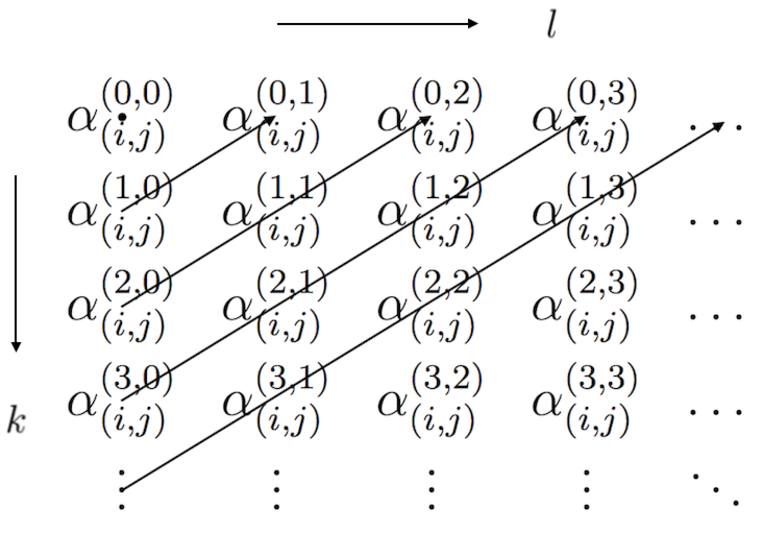
\includegraphics[width=70mm]{reordering_cropped.pdf}
			\captionsetup{justification=centering,margin=2cm}
			\captionof{figure}{}
			\label{fig:reordering}
		\end{figure}
		%\begingroup
		%\renewcommand*{\arraystretch}{1.5}
		%$$
		%\begin{matrix}
		%	\alpha^{(0,0)}_{(i,j)} & \alpha^{(0,1)}_{(i,j)} & \alpha^{(0,2)}_{(i,j)} & \alpha^{(0,3)}_{(i,j)} & \ldots \\
		%	\alpha^{(1,0)}_{(i,j)} & \alpha^{(1,1)}_{(i,j)} & \alpha^{(1,2)}_{(i,j)} & \alpha^{(1,3)}_{(i,j)} & \ldots \\
		%	\alpha^{(2,0)}_{(i,j)} & \alpha^{(2,1)}_{(i,j)} & \alpha^{(2,2)}_{(i,j)} & \alpha^{(2,3)}_{(i,j)} & \ldots \\
		%	\alpha^{(3,0)}_{(i,j)} & \alpha^{(3,1)}_{(i,j)} & \alpha^{(3,2)}_{(i,j)} & \alpha^{(3,3)}_{(i,j)} & \ldots \\
		%	\vdots & \vdots & \vdots & \vdots & \ddots
		%\end{matrix}
		%$$
		%\endgroup
		The equality holds as long as the original series is absolutely convergent, which is satisfied since every element of the matrix $e^{A+B}$ converges absolutely by Corollary \ref{cor:elementConvergence}.
	\end{enumerate}
\end{proof}

\begin{lemma}
	\label{lem:matrixExpIdentity}
	For any $a\in\K$ we have $e^{a I}=e^{a}I$.
\end{lemma}

\begin{proof}
	Follows straight from the definition of the matrix exponential.
	$$e^{a I}=\sum^\infty_{k=0}\frac{a^k}{k!}I^k=\left(\delta_{i,j}\sum^\infty_{k=0}\frac{a^k}{k!}\right)_{n\times n}=\left(\delta_{i,j}e^a\right)_{n\times n}=e^aI$$
\end{proof}

Now, using the properties in Lemma \ref{lem:expprop}, we can see that $\dot{x}(t)=Ax(t)$ is solved by $x(t)=e^{tA}x(0)$. The solution is unique which follows from the general theory of linear differential equations \cite[see][Věta 13.5.1]{Pick}.

\begin{claim}
\label{claim:uniqueness}
	The autonomous linear system $\dot{x}(t)=Ax(t)$ with an initial condition $x(0)$ is uniquely solved by $x(t)=e^{tA}x(0)$.
\end{claim}

\subsection{Stability of Linear Autonomous Systems}

Typically, we require the autonomous system to stabilize itself back into its stable state after some disturbances.

\begin{definition}
	The linear autonomous system $\dot{x}(t)=Ax(t)$ is \termdef{stable}, if for any initial state $x(0)\in\K^n$ the state vector $x(t)$ converges to $\nullvector$ for $t\to\infty$.
\end{definition}

Let $A$ be a real or complex matrix. Then there is a regular matrix $R\in \K^{n\times n}$ such that the matrix
$$J=R^{-1}AR$$
is in a Jordan normal form. By substituting $x(t)=Ry(t)$, which is equivalent to changing the basis of our system, we get 
\begin{align*}
	R\dot{y}(t)&=ARy(t) \\
	\dot{y}(t)&=R^{-1}ARy(t) \\
	\dot{y}(t)&=Jy(t)\ .
\end{align*}
Therefore, by Claim \ref{claim:uniqueness}, the unique solution is
$$y(t)=e^{tJ}y(0)\ .$$
It is sufficient to determine when $y(t)$ converges to \nullvector, because since $R$ is an invertible matrix, $x(t)$ converges to $\nullvector$ if and only if $y(t)$ converges to $\nullvector$.

We know that every Jordan block $J_{\lambda,n}$ in the matrix $J$ is of the form \linebreak $J_{\lambda,n}=\lambda I_n+N_n$, $n \in\N$, where $N_n=\left(n_{i,j}\right)_{n\times n}$ is the nilpotent matrix satisfying $n_{i,j}=\delta_{i,j-1}$. 
It is also true that $(N_n)^k_{i,j}=\delta_{i,j-k}$ and $(N_n)^n=O_{n \times n}$, since every right multiplication by the matrix $N$ shifts the multiplied matrix's columns to the right by one column, that is, it maps matrix $(v_1,\ldots,v_n)$ onto $(\nullvector,v_1,\ldots,v_{n-1})$. For example, in case of $n=4$ we have
\begin{equation*}
	N_4=
	\begin{pmatrix}
		0 & 1 & 0 & 0 \\
		0 & 0 & 1 & 0 \\
		0 & 0 & 0 & 1 \\
		0 & 0 & 0 & 0 
	\end{pmatrix},\ 
	(N_4)^2=
	\begin{pmatrix}
		0 & 0 & 1 & 0 \\
		0 & 0 & 0 & 1 \\
		0 & 0 & 0 & 0 \\
		0 & 0 & 0 & 0 
	\end{pmatrix},\ 
	(N_4)^3=
	\begin{pmatrix}
		0 & 0 & 0 & 1 \\
		0 & 0 & 0 & 0 \\
		0 & 0 & 0 & 0 \\
		0 & 0 & 0 & 0 
	\end{pmatrix}
	.
\end{equation*}

By Lemma \ref{lem:expprop}, for each Jordan block $J_{\lambda,n}$, we have
$$e^{tJ_{\lambda,n}}=e^{t(\lambda I_n + N_n)}=e^{t\lambda I_n}e^{tN}=e^{\lambda t}e^{tN_n}\ .$$
Let $\lambda = a+ib$ where $a$,$b \in \R$, then
$$e^{tJ_{\lambda,n}}=e^{at}e^{ibt}e^{tN}\ .$$
We know that $|e^{ibt}|=1$ and that
$$e^{tN}=\sum^\infty_{k=0}\frac{t^k}{k!}N^k=\sum^{n-1}_{k=0}\frac{t^k}{k!}N^k$$
since $(N_n)^n=O_{n \times n}$. Therefore, we can see that every element of the matrix $e^{tN}$ is a polynomial in $t$ of degree less than $n$. It follows that $e^{tJ_{\lambda,n}}$ approaches $O_{n \times n}$ for $t\rightarrow\infty$ if and only if
$$\lim_{t\to\infty}e^{at}t^{n-1}=0\ .$$
This holds for any $n\in\N$ if and only if $a<0$. 

Since any block diagonal matrix to the power of any natural number preserves its block form, we can write
\begin{equation*}
	J=
	\begin{pmatrix}
		J_{\lambda_1,n_1} & 0 & \cdots & 0 \\
		0 & J_{\lambda_2,n_2} & \cdots & 0 \\
		\vdots & \vdots & \ddots & \vdots \\
		0 & 0 & \cdots & J_{\lambda_r,n_r}
	\end{pmatrix},
	\quad 
	e^J=
	\begin{pmatrix}
		e^{J_{\lambda_1,n_1}} & 0 & \cdots & 0 \\
		0 & e^{J_{\lambda_2,n_2}} & \cdots & 0 \\
		\vdots & \vdots & \ddots & \vdots \\
		0 & 0 & \cdots & e^{J_{\lambda_r,n_r}}
	\end{pmatrix}
	,
\end{equation*}
where the zeroes in the matrices represent zero matrices of appropriate sizes. Therefore, since $y(0)$ is a constant vector, we see that $y(t)=e^{tJ}y(0)$ converges to $\nullvector$ if (and only if, because of the uniqueness of the solution) all the eigenvalues $\lambda_i$ of the matrix $A$ have negative real parts. As the last step, we calculate $x(t)=Ry(t)$ and $x(0)=Ry(0)$. Let us formulate this result into a theorem.

\begin{theorem}
\label{theorem:stability}
	The system $\dot{x}=Ax(t)$ is stable if and only if all eigenvalues of the matrix $A$ have negative real parts.
\end{theorem}

\subsection{Linear System With Control}

\begin{definition}
	A \termdef{continuous dynamic linear system with control u} is a system of linear differential equations of first order with constant coefficients in the form $$\dot{x}(t)=Ax(t)+Bu(t)\ ,$$ where the function $x(t)\colon\R^+\to\K^n$ is a \termdef{state vector} (\termdef{state} for short) of the system, $A\in\K^{n\times n}$ is a \termdef{fundamental matrix} of the system, $B\in\K^{n\times m}$ is a \termdef{control matrix} of the system and the continuous function $u(t)\colon\R^+\to\K^m$ is a \termdef{control vector} of the system. The \termdef{initial condition} of the system is the state $x(0)$.

	We will call this system the $(A,B)$ system for short.
\end{definition}

In a general case, this is called an \termdef{open-loop control} system because the control is not dependent on the previous state of the system.

We can imagine such a system as follows. The first summand of the right-hand side, $Ax(t)$, of the equation $\dot{x}(t)=Ax(t)+Bu(t)$ can be thought of as the model of the machine or the event that we want to control and the second summand, $Bu(t)$, as our control mechanism. The $B$ matrix fulfils the role of a ``control board'' and the control vector $u(t)$ is us deciding, which ``levers'' and ``buttons'' we want to push. 

Of course, if we want this system to be self-regulating, we cannot input our own values into $u(t)$, and therefore $u(t)$ has to be calculated from the current state of our system.

\begin{definition}
	Let us have a linear differential system with the control $u(t)$ defined as
	$$u(t)=Fx(t)\ ,$$
	where $F\in\K^{m\times n}$ is a \termdef{feedback matrix}. This system is then called a \termdef{closed-loop control} system or a \termdef{linear feedback control} system.

	For short, we will call this system the $(A,B,F)$ system.
\end{definition}

Usually, we are given an autonomous system and we need to find a feedback matrix $F$ such that the resulting system has some desired behavior. The feedback control system can be expressed as the linear autonomous system
$$\dot{x}(t)=Ax(t)+BFx(t)=(A+BF)x(t)\ .$$

\begin{definition}
	The linear feedback system $(A,B,F)$ is \termdef{stable}, if the linear autonomous system $\dot{x}(t)=(A+BF)x(t)$ is stable.
\end{definition}

By Theorem \ref{theorem:stability}, we now know that an $(A,B,F)$ system is stable if all eigenvalues of the matrix $A+BF$ have negative real parts. Therefore, we are left to provide a suitable feedback matrix $F \in \K^{n \times n}$. This requirement can also be expressed through the characteristic polynomial of the matrix $A~+~BF$, since the roots of the characteristic polynomial of a matrix are precisely eigenvalues of the matrix.

\begin{definition}
	Let $A$ be a $n\times n$ matrix. Then the \termdef{characteristic polynomial}~of~$A$, denoted by $\chi_A$, is defined as $$\chi_A(s)=\textnormal{det}(sI_n-A)\ .$$
\end{definition}

Through our observations we got to a conclusion, that we need to find a feedback matrix $F$ such that the characteristic polynomial of the matrix $A+BF$ is $$\chi_{A+BF}=(x-\lambda_1)(x-\lambda_2)\cdots(x-\lambda_n)\ ,$$ where all its roots $\lambda_1,\lambda_2,\ldots,\lambda_n \in \C$ have negative real parts. This leads to an important definition.

\begin{definition}
    Let $\K$ be a field and let $A \in \K^{n \times n}$, $B \in \K^{n \times m}$, $n,m \in \N$. We say that a polynomial $\chi$ is \termdef{assignable for the pair} $(A,B)$ if there exists such a matrix $F\in\K^{m \times n}$ that $$\chi_{A+BF}=\chi\ .$$
\end{definition}

The pole shifting theorem states, that if $A$ and $B$ are ``sensible'' in a sense that we will discuss in the next section, then an arbitrary monic polynomial $\chi$ of degree $n$ can be assigned to the pair $(A,B)$. It also claims that it is immaterial over what field $A$ and $B$ are.

\section{Controllable pairs}

In this section we will establish the notion of controllability. We will first explain this concept for \textit{discrete-time systems} and then we will show that the requirement for controllability of \textit{continuous-time systems} is the same as the one for \textit{discrete-time systems}.

\subsection{Discrete-time systems}

Let us have a continuous dynamic system $\dot{x}(t)=A_1x(t)$, where $A_1$ is a real or complex square matrix. We \textit{discretize} the time, that is, instead of using continuous real-time values of $x(t)$ and $\dot{x}(t)$, we are interested in these values only at discrete \textit{sampling times} $0,\delta,2\delta,\ldots,k\delta,\ldots$ where $\delta\in\R^+$. We will denote the states at each sampling time as
$$x_k=x(k\delta)\ ,k\in\N_0\ .$$
The solution of this system is by Theorem \ref{claim:uniqueness} precisely $x(t)=e^{tA_1}x(0)$. For some fixed $k\in\N$ we get $x_k=x(k\delta)=e^{k\delta A_1}x(0)$. Using the fourth point of Lemma \ref{lem:expprop} we obtain 
\begin{align*}
	x_{k+1}
	&=e^{(k+1)\delta A_1}x(0) \\
	&=e^{\delta A_1 +k\delta A_1}x(0) \\
	&=e^{\delta A_1}e^{k\delta A_1}x(0) \\
	&=e^{\delta A_1}x_k \\
	&=Ax_k
\end{align*}
by choosing $A=e^{\delta A_1}$. We see that the value of $x$ at the sample time $k$ can be calculated from its previous value. We will now define such a system. The definition holds for any field $\K$.

\begin{definition}
	Let $\K$ be a field. A \termdef{discrete dynamic linear system} is a system of equations
	$$x_{k+1}=Ax_k,\ k\in\N_0\ ,$$
	where $x_k\in \K^n$ is a \termdef{state vector} (\termdef{state} for short) of the system and the matrix $A\in \K^{n\times n}$ is a \termdef{fundamental matrix} of the system. The \termdef{initial condition} of the system is the state $x(0)$.
\end{definition}

Similarly, we can define a discrete dynamic linear system with control.

\begin{definition}
	Let $\K$ be a field. A \termdef{discrete dynamic linear system with control u} is a system of equations
	$$x_{k+1}=Ax_k+Bu_k,\ k\in\N_0\ ,$$
	where $x_k\in\K^n$ is a \termdef{state vector} (\termdef{state} for short) of the system, $A\in\K^{n\times n}$ is a fundamental matrix, $B\in\K^{n\times m}$ is a control matrix and $u_k\in\K^m$ is a control vector. The \termdef{initial condition} of the system is the state $x_0$.

	We will call this system the \termdef{discrete $(A,B)$} system.
\end{definition}

\begin{definition}
	Let $(A,B)$ be a discrete system. We say that a state $x$ can be \termdef{reached} in a time $k\in\N_0$ if there exists such a sequence of control vectors $u_0,u_1,\ldots,u_{k-1}$ that for the initial condition $x_0=\nullvector$ we get $x=x_k$.
\end{definition}

\sloppy
States that can be reached in time $k\in\N$ in open-loop control discrete-time systems can be derived as follows. The initial condition is $x_0=\nullvector$ and we can choose arbitrary $u_0,u_1,\ldots,u_{k-1}$. Then for $k=1$ we have 
$$x_1=Ax_0+Bu_0=Bu_0 \in \text{Im}B\ .$$
For $k=2$ we get
$$x_2=Ax_1+Bu_1=ABu_0+Bu_1\in\text{Im}(AB|B)\ .$$
It is clear, that for every $k\in\N$ it holds
$$x_k\in\text{Im}(A^{k-1}B|\cdots|AB|B)\ .$$
For every $k\in\N$ it is also true that
$$\text{Im}(B|AB|\cdots|A^kB) \subseteq \text{Im}(B|AB|\cdots|A^{k+1}B)\ .$$
By the Cayley–Hamilton theorem we know that $\chi_A(A)=O_{n\times n}$. That means, that $A^n$ can be expressed as a linear combination of the matrices $\{I,A,\ldots,A^{n-1}\}$ which implies that $A^nB$ can be expressed as a linear combination of the matrices $\{B,AB,\ldots,A^{n-1}B\}$. We now see that $$\text{Im}(B|AB|\cdots|A^{n}B) \subseteq \text{Im}(B|AB|\cdots|A^{n-1}B)\ .$$
It follows
\begin{equation}
\label{eq:cayleHamilReachable}
	\text{Im}(B|AB|\cdots|A^{n-1}B)=\text{Im}(B|AB|\cdots|A^{n-1}B|A^nB)\ .
\end{equation}
For an arbitrary $k\in\N,k>n$ we have $$A^kB=A^{k-n}A^nB=A^{k-n}\sum^{n-1}_{i=0}\alpha_i A^iB=\sum^{n-1}_{i=0}\alpha_i A^{k-n+i}B\in\text{Im}(B|AB|\ldots|A^{k-1}B)\ ,$$
for some $\alpha_0,\ldots,\alpha_{n-1}\in\K$.
Therefore, by induction, all the states we could reach in any time $k\in\N$ are already in the space 
$$\text{Im}(B|AB|\cdots|A^{n-1}B)\ .$$
\begin{definition}
	Let $\K$ be a field and let $A \in \K^{n \times n}$, $B \in \K^{n \times m}$, $n,m \in \N$. The matrix $$\mathbf{R}(A,B)=(B|AB|\cdots|A^{n-1}B)$$ is called the \termdef{rechability matrix} of $(A,B)$. We define the \termdef{reachable space} $\mathcal{R}(A,B)$ of the pair $(A,B)$ as $\text{Im}(\mathbf{R}(A,B))$. 
\end{definition}
TODODO
\begin{definition}
	Let $\K$ be a field, $\mathcal{V} \subseteq \K^n$ be a vector space and let $A\in\K^{m\times n}$. Then we define the product of the left multiplication of the space $\mathcal{V}$ by the matrix $A$ as the set $A\cdot\mathcal{V}=A\mathcal{V}=\{Av|v\in\mathcal{V}\}$.
\end{definition}

We have seen that by left multiplying $\mathcal{R}(A,B)$ by $A$, we get a subspace which is already included in $\mathcal{R}(A,B)$. This leads to an important property of some subspaces.

\begin{definition}
	Let $V$ be a vector space, $W$ be its subspace and let $f$ be a mapping from $V$ to $V$. We call $W$ an \termdef{invariant subspace} of $f$ if $f(W)\subseteq W$. We also say that $W$ is \termdef{$f$-invariant}. 
	
	If $f=f_A$ for some matrix $A$, we also say that W is \termdef{$A$-invariant} for short.
\end{definition}

\begin{lemma}
	\label{lem:reachinv}
	$\mathcal{R}(A,B)$ is an $A$-invariant subspace.
\end{lemma} 

\begin{proof}
	It follows from the discussion above.
\end{proof}

This leads us to an important property of the pair $(A,B)$. We want to be able to get the system into any state by controlling it with our control $u$, i.e., choosing an appropriate sequence $u_0,\ldots,u_{n-1}$. Therefore, we desire that $\mathcal{R}(A,B)=\K^n$. An equivalent condition is $\text{dim}\mathcal{R}(A,B)=n$.

\begin{definition}
	Let $\K$ be a field and let $A \in \K^{n \times n}$, $B \in \K^{n \times m}$, $n,m \in \N$. The pair $(A,B)$ is \termdef{controllable} if $\textnormal{dim}\mathcal{R}(A,B)=n$.
\end{definition}

\subsection{Continuous-time systems}

\begin{remark}
	In this section we assume, that $\K$ is a field of either real or complex numbers and that $A\in\K^{n\times n}$, $B\in\K^{n\times m}$.
\end{remark}

We will now show that the condition for controllability of discrete-time systems also characterizes controllable continuous-time systems. In order to prove this idea, we will express the solution of such a system as a linear combination of the matrices $A^iB$, for $i\in \N_0$.

\begin{definition}
	Let us have a vector function $v(t)\colon\R\to\K^n$. Then the definite integral of the function on an interval $[a,b]$, $a,b\in\R$ is
	$$\int_a^bv(t)dt=\left(\int_a^bv_1(t)dt\ ,\ \ldots\ ,\ \int_a^bv_n(t)dt\right)^T\ .$$
\end{definition}

\begin{lemma}
\label{lem:matrixTimesVectorDerivative}
	For a matrix function $A(t)\colon\R\to\K^{n\times m}$ and a vector function $v(t)\colon\R\to\K^m$ it holds 
	$$\frac{d}{dt}\left(A(t)v(t)\right)=\left(\frac{d}{dt}A(t)\right)v(t)+A(t)\frac{d}{dt}v(t)$$
\end{lemma}

\begin{proof}
	Can be simply shown by rewriting the vector $A(t)v(t)$ elementwise.
\end{proof}

We utilize the matrix exponential in solving the inhomogeneous linear system $\dot{x}(t)=Ax(t)+Bu(t)$. By left multiplying it by $e^{-tA}$ we get
\begin{align*}
	e^{-tA}\dot{x}(t)-e^{-tA}Ax(t) &=e^{-tA}Bu(t) \\
	\frac{d}{dt} (e^{-tA}x(t)) &=e^{-tA}Bu(t)\ .
\end{align*}
Note that we used Lemma \ref{lem:matrixTimesVectorDerivative} and the equality $e^{-tA}A=Ae^{-tA}$, following from the first point of Lemma \ref{lem:expprop}. After integrating both sides with respect to $t$ on interval $(t_0,t_1)$ we obtain
\begin{align*}
	[e^{-tA}x(t)]^{t_1}_{t_0}&=\int^{t_1}_{t_0}e^{-tA}Bu(t)dt \\
	e^{-t_1A}x(t_1)-e^{-t_0A}x(t_0)&=\int^{t_1}_{t_0}e^{-tA}Bu(t)dt \\
	x(t_1)&=e^{(t_1-t_0)A}x(t_0)+\int^{t_1}_{t_0}e^{(t_1-t)A}Bu(t)dt\ .
\end{align*}
The integral makes sense since $u(t)$ is required to be continuous.

Now it is clear that in the system where $x(0)=\nullvector$, the state in time $t\in \R^+$ is equal to
\begin{equation}
\label{eq:coolVzorec}
	x(t)=\int^t_0 e^{(t-s)A}Bu(s)ds\ .
\end{equation}

\begin{definition}
	We say that a state $x\in\K^n$ can be \termdef{reached in time $t$}, if there exists a control $u(x)\colon[0,t]\rightarrow\K^m$ such that
	$$x=\int^t_0 e^{(t-s)A}Bu(s)ds\ .$$

	The set of all states that can be reached in time $t$ is denoted by $\mathcal{R}^t$. The set $\mathcal{R}=\cup_{t\in\R^+}\mathcal{R}^t$ of all states that can be reached, is called a \termdef{reachable space}.
\end{definition}

\begin{definition}
	An $n$-dimensional continuous-time linear system is \termdef{controllable}, if $\mathcal{R}=\K^n$.
\end{definition}

\begin{theorem}
	The $n$-dimensional continuous-time linear system is controllable if and only if $\text{dim}\mathcal{R}(A,B)=n$.
\end{theorem}

\begin{proof}
	From the discussion above we have 
	$$
		x(t)=\int^t_0e^{(t-s)A}Bu(s)ds
		=\int^t_0\sum^\infty_{k=0}\frac{(t-s)^k}{k!}A^kBu(s)ds\ .
	$$
	The $n$-dimensional vector $w^{(k)}(s)=A^kBu(s)$ has the elements
	$$w^{(k)}_i(s)=\sum^m_{j=1}\alpha^{(k)}_{i,j}u_j(s)\ ,$$
	where $\alpha^{(k)}_{i,j}$ is the element of the matrix $A^kB$ on the position $(i,j)$. Therefore, the $i$-th element of $x(t)$ is equal to
	$$
		x_i(t)
		=\int^t_0\sum^\infty_{k=0}\frac{(t-s)^k}{k!}w^{(k)}_ids
		=\int^t_0\sum^\infty_{k=0}\sum^m_{j=1}\frac{(t-s)^k}{k!}\alpha^{(k)}_{i,j}u_j(s)ds\ .
	$$
	
	Now, in order to be able to modify this expression, we will prove that the series $\sum^\infty_{k=0}\frac{(t-s)^k}{k!}\alpha^{(k)}_{i,j}u_j(s)$ is absolutely convergent for every position $(i, j)$. Following from Lemma \ref{lem:elementAbsoluteSize}, we have
	\begin{equation*}
		\sum^N_{k=0}\abs{\frac{(t-s)^k}{k!}\alpha_{i,j}^{(k)}u_j(s)}\leq \sum^N_{k=0}\frac{\abs{t-s}^k}{k!}\abs*{\alpha_{i,j}^{(k)}}\abs*{u_j(s)}\leq\abs*{u_j(s)}\norm{B}_F\sum^N_{k=0}\frac{\norm{(t-s)A}_F^k}{k!}\ .
	\end{equation*}
	This gives us
	$$\sum^\infty_{k=0}\abs{\frac{(t-s)^k}{k!}\alpha_{i,j}^{(k)}u_j(s)}=\lim_{N\to\infty}\sum^N_{k=0}\abs{\frac{(t-s)^k}{k!}\alpha_{i,j}^{(k)}u_j(s)}\leq \abs*{u_j(s)}\norm{B}_Fe^{\norm{(t-s)A}_F}\ .$$
	Because of the absolute convergence, we can now swap the integral and the series:
	\begin{align*}
		x_i(t)
		&=\int^t_0\sum^\infty_{k=0}\sum^m_{j=1}\frac{(t-s)^k}{k!}\alpha^{(k)}_{i,j}u_j(s)ds
		=\sum^\infty_{k=0}\int^t_0\sum^m_{j=1}\frac{(t-s)^k}{k!}\alpha^{(k)}_{i,j}u_j(s)ds
		\\
		&=\sum^\infty_{k=0}\sum^m_{j=1}\int^t_0\frac{(t-s)^k}{k!}\alpha^{(k)}_{i,j}u_j(s)ds
		=\sum^\infty_{k=0}\sum^m_{j=1}\frac{\alpha^{(k)}_{i,j}}{k!}\int^t_0(t-s)^ku_j(s)ds
		\\
		&=\sum^\infty_{k=0}\sum^m_{j=1}\frac{\alpha^{(k)}_{i,j}}{k!}v^{(k)}_j(t)\ ,
	\end{align*}
	where $v^{(k)}(t)=\int^t_0(t-s)^ku(s)ds$ is a vector of length $m$. Therefore, we have 
	$$x(t)=\sum^\infty_{k=0}\frac{1}{k!}A^kBv^{(k)}(t)=\sum^\infty_{k=0}\frac{1}{k!}A^kB\int^t_0(t-s)^ku(s)ds\ .$$
	By the Cayley-Hamilton theorem it then holds
	\begin{align*}
		x(t)
		&=\sum^\infty_{k=0}\frac{1}{k!}A^kBv^{(k)}(t)
		=\sum^\infty_{k=0}\frac{1}{k!}\left(\sum^{n-1}_{j=0}\alpha_{k,j}A^j\right)Bv^{(k)}(t)
		\\
		&=\sum^\infty_{k=0}\sum^{n-1}_{j=0}\frac{1}{k!}\alpha_{k,j}A^jBv^{(k)}(t)
		=\sum^{n-1}_{j=0}\sum^\infty_{k=0}\frac{1}{k!}\alpha_{k,j}A^jBv^{(k)}(t)
		\\
		&=\sum^{n-1}_{j=0}\sum^\infty_{k=0}A^jB\left(\frac{1}{k!}\alpha_{k,j}v^{(k)}(t)\right)
		=\sum^{n-1}_{j=0}A^jB\sum^\infty_{k=0}\left(\frac{1}{k!}\alpha_{k,j}v^{(k)}(t)\right)
		\ .
	\end{align*}
	The fourth equality follows from the absolute convergence of the resulting series, which can be shown in a similar way as above. 

	Now we see that $$x(t) \in \text{Im}(B|AB|\ldots|A^{n-1}B)=\mathcal{R}(A,B)\ .$$ 
	
	If the system is controllable, then $x(t)$ can be equal to any of the vectors of an arbitrary basis of $\K^n$. Therefore, we know that $n$ linearly independent vectors belong into $\mathcal{R}(A,B)$, and it follows that $\text{dim}\mathcal{R}(A,B)=n$.

	For the proof of the ``if'' part we use \citet[Theorem 3]{Sontag1998}.

	Conversely, if controllability fails, then there exists a non-trivial complement $\mathcal{S}$ to the reachable space $\mathcal{R}$. For any time $t\in\R^+$ and any vector $\rho\in\mathcal{S}$ it holds that $\rho^\ast x(t)=\nullvector$. By choosing the control $u(t)=B^\ast e^{(t-s)A^\ast}\rho$, which is continuous, on the interval $[0,s]$, we get by the equation (\ref{eq:coolVzorec})
	$$\nullvector=\rho^\ast x(t)=\int^t_0\rho^\ast e^{(t-s)A}BB^\ast e^{(t-s)A^\ast}\rho ds=\int^t_0\norm{B^\ast e^{(t-s)A^\ast}\rho}^2\ .$$
	This implies
	$$0=\norm{B^\ast e^{(t-s)A^\ast}\rho}^2=\norm{\rho^\ast e^{(t-s)A}B}^2$$
	and hence
	$$\nullvector=\rho^\ast e^{(t-s)A}B=\sum^\infty_{k=0}\frac{(t-s)^k}{k!}\rho^\ast A^kB\ .$$
	This implies, by similar usage of Cayley-Hamilton as in the ``only if'' part of the proof, that the vector $\rho$ is perpendicular to $\mathcal{R}(A,B)$ and therefore $\text{dim}\mathcal{R}(A,B)$ cannot be equal to $n$.
\end{proof}

\subsection{Decomposition theorem}

\begin{lemma}
	\label{lem:invsubspc}
	Let $W$ be an invariant subspace of a linear mapping $f\colon V \rightarrow V$. Then there exists a basis $C$ of $V$ such that 
	\begin{equation*}
		[f]^C_C=
		\begin{pmatrix}
			F_1 & F_2 \\
			0   & F_3 
		\end{pmatrix}\ ,
	\end{equation*}
	where $F_1$ is $r\times r$, $r=\text{dim}W$.
\end{lemma}

\begin{proof}
	Let $(w_1,\ldots,w_r)$ be an arbitrary basis of the subspace $W$. We complete this sequence into basis $C$ of $V$ with vectors $v_1,\ldots,v_{n-r}$ where $n=\text{dim}V$, thus $C=(w_1,\ldots,w_r,v_1,\ldots,v_{n-r})$. We know that
	$$[f]^C_C=([f(w_1)]_C,\ldots,[f(w_r)]_C,[f(v_1)]_C,\ldots,[f(v_{n-r})]_C)\ .$$
	Since $W$ is an $A$-invariant subspace, it holds that $f(w_i)\in W$ and therefore, because of our choice of the basis $C$, the matrix $[f]^C_C$ is of the desired form.
\end{proof}

If $(A,B)$ is not controllable, then there exists a part of the state space that is not affected by the input. This can be shown using the following theorem.

\begin{theorem}
	\label{theorem:decomp}
	Let $\K$ be a field, $(A,B)$ be a dynamic system over $\K$ and let $\text{dim}\mathcal{R}(A,B)=r\leq n$. Then there exists an invertible $n\times n$ matrix $T$ over $\K$ such that the matrices $\widetilde{A}:=T^{-1}AT$ and $\widetilde{B}:=T^{-1}B$ have the block structures 
	\begin{equation}
		\label{eq:decomp}
		\widetilde{A}=
		\begin{pmatrix}
			A_1 & A_2 \\
			0   & A_3 
		\end{pmatrix}
		\qquad
		\widetilde{B}=
		\begin{pmatrix}
			B_1  \\
			0
		\end{pmatrix}\ ,
	\end{equation}
	where $A_1\in\K^{r \times r}$ and $B_1\in\K^{r \times m}$.
\end{theorem}

\begin{proof}
	We know that $\mathcal{R}(A,B)$ is an $A$-invariant subspace (Lemma \ref{lem:reachinv}). Using Lemma \ref{lem:invsubspc} on the matrix mapping $f_A$ we get a basis $C$ for which it holds that 
	$$[f_A]^C_C=[\text{id}]^K_C[f_A]^K_K[\text{id}]^C_K=[\text{id}]^K_CA[\text{id}]^C_K$$ 
	is in a block upper triangular form. By putting $T=[\text{id}]^C_K$ we get that $\widetilde{A}=[f_A]^C_C$ is in the desired form.

	Now, let us consider the matrix mapping $f_B$. We have
	$$\widetilde{B}=TB=[\text{id}]^{K_n}_C[f_B]^{K_m}_{K_n}=[f_B]^{K_m}_C=([f_B(e_1)]_C,\ldots,[f_B(e_m)]_C)\ .$$
	Since $f_B(e_i)$ is the $i$-th column of the matrix $B$, and trivially by definition of a reachable space it holds that $\text{Im}(B)\subseteq \mathcal{R}(A,B)$, we see that $\widetilde{B}$ is in the requested form.
\end{proof}

We achieved the new form of matrices $A$ and $B$ by changing the basis of our state space. We now define the relation between $(A,B)$ and $(\widetilde{A},\widetilde{B}).$

\begin{definition}
	Let $(A,B)$ and $(\widetilde{A},\widetilde{B})$ be pairs as the ones described in Theorem \ref{theorem:decomp}. Then $(A,B)$ \termdef{is similar to} $(\widetilde{A},\widetilde{B})$, denoted $(A,B) \sim (\widetilde{A},\widetilde{B})$, if there exists an invertible matrix $T$ for which it holds that
	$$\widetilde{A}=T^{-1}AT\quad and\quad\widetilde{B}=T^{-1}B\ .$$
\end{definition}

\begin{lemma}
	\label{lem:simMatrices}
	Let $A$ and $B$ be similar matrices, that is, there exists an invertible matrix $R$ such that $A=R^{-1}BR$. Then $\chi_A=\chi_B$.
\end{lemma}

\begin{proof}
	We will use properties of the matrix determinant:
	\begin{align*}
		\chi_A&=\text{det}(sI-A)=\text{det}(sI-R^{-1}BR) \\
		&=\text{det}(sR^{-1}IR-R^{-1}BR)=\text{det}(R^{-1}(sI-B)R) \\
		&=(\text{det}R)^{-1}\text{det}(sI-B)\text{det}R=\text{det}(sI-B) \\
		&=\chi_B\ .
	\end{align*}
\end{proof}

\begin{lemma}
	\label{lem:simPairsAssignablePolynomial}
	If $(A,B)\sim(\widetilde{A},\widetilde{B})$, then the assignable polynomials for the pairs $(A,B)$ and $(\widetilde{A},\widetilde{B})$ are the same.
\end{lemma}

\begin{proof}
	Let $T$ be a regular matrix over $\K$ such that $\widetilde{A}=T^{-1}AT$ and $\widetilde{B}=T^{-1}B$. Then for any feedback matrix $F$ we have 
	$$T^{-1}(A+BF)T=T^{-1}ATT^{-1}BFT=\widetilde{A}+\widetilde{B}\widetilde{F}\ ,$$
	where $\widetilde{F}=FT$. It follows from Lemma \ref{lem:simMatrices} that $$\chi_{A+BF}=\chi_{\widetilde{A}+\widetilde{B}\widetilde{F}}\ .$$
\end{proof}

Theorem \ref{theorem:decomp} has the following interesting consequence. Let $(A,B)$ be a dynamic system with the initial condition $x(0)=\nullvector$, and let $T$ be a regular matrix over $\K$ as in Theorem \ref{theorem:decomp}. By putting $x(t)=Ty(t)$ we get 
$$T\dot{y}(t)=ATy(t)+Bu(t)\ ,$$ 
which can be rewriten as 
$$\dot{y}(t)=T^{-1}ATy(t)+T^{-1}Bu(t)=\widetilde{A}y(t)+\widetilde{B}u(t)\ .$$ 
This gives us 
\begin{alignat*}{3}
	\dot{y}_1(t)&=A_1y_1(t)+&A_2y_2(t)&+B_1u(t)& \\
	\dot{y}_2(t)&=&A_3y_2(t)&&\ ,
\end{alignat*}
where $y(t)=(y_1(t),y_2(t))^T$, $y_1(t)\in\K^r$ and $y_2(t)\in\K^{n-r}$. The component $y_2(t)$ cannot be controlled and it is, for the initial condition $y(0)=Tx(0)=\nullvector$, always equal to \nullvector, since it does not depend on the control vector $u(t)$. 

It is also true that the system $(A_1,B_1)$ from Theorem \ref{theorem:decomp} is a controllable pair, which we will state as a lemma.

\begin{lemma}
	\label{lem:A_1B_1controllable}
	The pair $(A_1,B_1)$ is controllable.
\end{lemma}

\begin{proof}
	We know that $\text{dim}\mathcal{R}(A,B)=r$. We desire that $\text{dim}\mathcal{R}(A_1,B_1)=r$. We will show that $\text{dim}\mathcal{R}(A,B)=\text{dim}\mathcal{R}(\widetilde{A},\widetilde{B})=\text{dim}\mathcal{R}(A_1,B_1)$. 
	First, we have 
	\begin{align*}
		\mathcal{R}(\widetilde{A},\widetilde{B})&=\text{Im}(\widetilde{A}^{n-1}\widetilde{B}|\cdots|\widetilde{A}\widetilde{B}|\widetilde{B}) \\
		&=\text{Im}((T^{-1}AT)^{n-1}T^{-1}B|\cdots|T^{-1}ATT^{-1}B|T^{-1}B) \\
		&=\text{Im}(T^{-1}A^{n-1}B|\cdots|T^{-1}AB|T^{-1}B) \\
		&=\{(T^{-1}A^{n-1}B|\cdots|T^{-1}AB|T^{-1}B)\cdot v | v \in \K^{n\cdot m}\} \\
		&=\{T^{-1}(A^{n-1}B|\cdots|AB|B)\cdot v | v \in \K^{n\cdot m}\} \\
		&=T^{-1}\cdot\{(A^{n-1}B|\cdots|AB|B)\cdot v | v \in \K^{n\cdot m}\} \\
		&=T^{-1}\cdot(\text{Im}(A^{n-1}B|\cdots|AB|B)) \\
		&=T^{-1}\cdot(\mathcal{R}(A,B))
		\ .
	\end{align*}
	Since $T$ is an invertible matrix, which preserves linear independence, we have
	$$\text{dim}\mathcal{R}(\widetilde{A},\widetilde{B})=\text{dim}(T^{-1}\mathcal{R}(A,B))=\text{dim}(\mathcal{R}(A,B))=r\ .$$

	Now let us focus on the structure of $\mathcal{R}(\widetilde{A},\widetilde{B})$. We know that the last $n-r$ rows of $\widetilde{B}$ are equal to $\nullvector$. Also, because of the structure of $\widetilde{A}$, for an arbitrary matrix $X\in\K^{r\times m}$ we have that 
	\begin{equation*}
		\widetilde{A}
		\begin{pmatrix}
			X \\
			0
		\end{pmatrix}
		=
		\begin{pmatrix}
			A_1 & A_2 \\
			  0 & A_3
		\end{pmatrix}
		\begin{pmatrix}
			X \\
			0
		\end{pmatrix}
		=
		\begin{pmatrix}
			A_1X \\
			0
		\end{pmatrix}\ ,
	\end{equation*}
	where, again, the last $n-r$ rows are equal to $\nullvector$. Therefore, for any positive integer $k$ we have 
	\begin{equation*}
		\widetilde{A}^k\widetilde{B}=
		\begin{pmatrix}
			A_1^{k}B_1 \\
			0
        \end{pmatrix}
        \ ,A_1^kB_1\in\K^{r\times r}\ .
    \end{equation*}
    It follows
    \begin{equation*}
        \mathcal{R}(\widetilde{A},\widetilde{B})=
        \begin{pmatrix}[c|c|c|c]
            \begin{pmatrix}
                A_1^{n-1}B_1 \\
                0 
            \end{pmatrix}
            & \cdots &
            \begin{pmatrix}
                A_1B_1 \\
                0 
            \end{pmatrix}
            &
            \begin{pmatrix}
                B_1 \\
                0 
            \end{pmatrix}
        \end{pmatrix}\ .
    \end{equation*}
	
	By the equality (\ref{eq:cayleHamilReachable}) we have that the restriction to the first $r$ coordinates of $\mathcal{R}(\widetilde{A},\widetilde{B})$ is equal to $\mathcal{R}(A_1,B_1)$. Finally, it follows that
	$$\text{dim}\mathcal{R}(A_1,B_1)=\text{dim}\mathcal{R}(\widetilde{A},\widetilde{B})=\text{dim}\mathcal{R}(A,B)=r\ .$$
\end{proof}

Now we can see that the decomposition described in Theorem \ref{theorem:decomp} decomposes the matrix $A$ into the ``controllable'' and the ``uncontrollable'' parts $A_1$ and $A_3$ respectively.

\begin{cor}
	Let $(A,B)$ be a dynamic system, and let $T$ be a regular matrix and $\widetilde{A}=T^{-1}AT$ as in Theorem \ref{theorem:decomp}. Then it holds
	$$\chi_A=\chi_{\widetilde{A}}=\chi_{A_1}\chi_{A_3}=\chi_c\chi_u\ .$$
\end{cor} 

\begin{proof}
	Follows from Theorem \ref{theorem:decomp} and Lemma \ref{lem:simMatrices}.
\end{proof}

\begin{definition}
	The polynomials $\chi_c$ and $\chi_u$ are respectively the \termdef{controllable} and the \termdef{uncontrollable parts} of the characteristic polynomial $\chi_A$ with respect to the pair $(A,B)$. In the case where $r=0$ we put $\chi_c=1$, and in the case where $r=n$ we put $\chi_u=1$.
\end{definition}

For this definition to be correct, we need to show that polynomials $\chi_{A_1}$ and $\chi_{A_3}$ are not dependent on the choice of the regular matrix $T$ from Theorem \ref{theorem:decomp}. Since $\chi_{A_3}=\chi_A/\chi_{A_1}$, it is sufficient only to show that $\chi_{A_1}$ is independent of the choice.

\begin{lemma}
	Let A be a square matrix over $\K$. Then the controllable part $\chi_c$ of its characteristic polynomial is independent of the choice of the basis for $\mathcal{R}(A,B)$.
\end{lemma}

\begin{proof}
	Let $C=(c_1,\ldots,c_n)$ and $D=(d_1,\ldots,d_n)$ be two bases for $\K^n$ as constructed in the proof of Theorem \ref{theorem:decomp}. Then we have 
	\begin{equation*}
		[f_A]^C_C=
		\begin{pmatrix}
			A_1 & A_2 \\
			0   & A_3
		\end{pmatrix}\ ,
		\quad
		[f_A]^D_D=
		\begin{pmatrix}
			A_1' & A_2' \\
			0    & A_3'
		\end{pmatrix}\ ,
	\end{equation*}
	as in (\ref{eq:decomp}).
	We want to show that $\chi_{A_1}=\chi_{A_1'}$.

	It is true that
	$$[f_A]^C_C=[id]^D_C[f_A]^D_D[id]^C_D\ ,$$
	where
	$$[id]^C_D=([c_1]_D,\ldots,[c_n]_D)\ .$$
	We know that the vectors $c_1,\ldots,c_r$ form a basis of the subspace $\mathcal{R}(A,B)$ and that the vectors $d_1,\ldots,d_r$ form another basis of the same subspace. Therefore
	\begin{equation*}
		[id]^C_D=
		\begin{pmatrix}
			T_1 & T_2 \\
			0   & T_3
		\end{pmatrix}\ ,
		\quad
		[id]^D_C=([id]^C_D)^{-1}=
		\begin{pmatrix}
			T_1^{-1} & X \\
			0        & T_3^{-1}
		\end{pmatrix}\ ,
	\end{equation*}
	where $T_1\in\K^{r\times r}$ is a regular matrix, $T_3\in\K^{n-r\times n-r}$ and $T_2,X\in\K^{r\times n-r}$. It follows 
	\begin{equation*}
		\begin{pmatrix}
			A_1 & A_2 \\
			0   & A_3
		\end{pmatrix}
		=
		\begin{pmatrix}
			T_1^{-1} & X \\
			0        & T_3^{-1}
		\end{pmatrix}
		\begin{pmatrix}
			A_1' & A_2' \\
			0    & A_3'
		\end{pmatrix}
		\begin{pmatrix}
			T_1 & T_2 \\
			0   & T_3
		\end{pmatrix}\ ,
	\end{equation*}
	which implies that
	$$A_1=T_1^{-1}A_1'T_1\ .$$
	By Lemma \ref{lem:simMatrices} it then holds that $\chi_{A_1}=\chi_{A_1'}$.
\end{proof}